\chapter{Event Cameras}\label{sec:evtcams}

\section{Introduction}
Event cameras --- also known as neuromorphic cameras, dynamic vision sensors, or silicon retinas --- are novel, biologically-inspired sensors. Compared to traditional cameras, the specific architecture of the event cameras allows them to perceive highly dynamic scenes with low latency and with high dynamic range. Thanks to these properties, they represent a sensor of interest to answer the limitations encountered by the use of more traditional sensors in complex conditions.

Even though the first concept of an event camera was proposed over 30 years ago~\cite{Mahowald1991TheSR,Mahowald1992VLSIAO}, this sensor has gained traction within the scientific community over the past decade. This rise in popularity is especially due to their easier access, with the arrival of commercial sensors (especially all-in-one frame- and event-based sensors like the DAVIS~\cite{Brandli2014A2}), and with a growing number of software and development kits.

Due to their central position, this first chapter of the thesis is dedicated to an in-depth review of the event camera. We explain here its core concepts, describe its advantages and challenges, and quickly review the state of the art.

\section{Core Principle}
In a traditional camera, an image is captured by accumulating light during a short period of time (the \textit{exposure time}). Each pixel is then assigned an intensity value based on the amount of light received. All pixels are synchronously controlled by a single global clock, and images are outputted at a predefined frame rate (e.g., 30\acrshort{fps}).

In opposition, in an event camera, all pixels are independent units. Each pixel responds to changes in the log-irradiance (or ``brightness'') it receives. More specifically, if we note the brightness \(L \doteq \log(E)\) (where \(E\) is the irradiance), then an event \(e \doteq (\mathbf{x}, t, p)\) is triggered at a pixel \(\mathbf{x} \doteq (x, y)\) and at time \(t\) if the brightness difference since the last event at that pixel, i.e., if

\begin{equation}\label{eq:evtcams:delta_l}
  \Delta L(\mathbf{x}, t) \doteq L(\mathbf{x}, t) - L(\mathbf{x}, t - \Delta t)
\end{equation}

crosses a threshold \(\delta\), i.e.,

\begin{equation}\label{eq:evtcams:delta_l_thr}
  |\Delta L(\mathbf{x}, t)| \geq \delta
\end{equation}

where \(\delta > 0\), and where \(\Delta t\) is the amount of time since the last event at that pixel. The polarity \(p\) of the event can then be defined as the sign of the brightness difference, i.e.,

\begin{equation}
  p \doteq \sign(\Delta L(\mathbf{x}, t))
\end{equation}

For an easier understanding, an illustration of these equations is given in \cref{fig:evtcams:intensity_evts}.

\begin{figure}[t]
  \centering
  \begin{tikzpicture}
    \begin{axis}[axis equal image,
                 axis lines=left,
                 xlabel={Time}, ylabel={\(\log(E)\)},
                 x label style={at={(axis description cs:1.1,0.125)},anchor=north},
                 y label style={at={(axis description cs:0.0,1.0)},rotate=-90,anchor=south},
                 xmin=0, xmax=13.5, ymin=0, ymax=4.5,
                 xtick distance=50, ytick distance=50,
                 xticklabels={}, yticklabels={},
                 extra x ticks={1,2,3,5,10,12}, extra x tick labels={}]
      \addplot[smooth, mark=none] table [x=t, y=log_i, col sep=comma] {mainmatter/plots/2_event_cameras/intensity_evts/intensity_evts.csv};
      % Uncomment the following line if you want to add the reconstruction to the plot
      %\addplot[const plot, mark=none, densely dashed] table [x=t, y=log_i_const, col sep=comma] {mainmatter/plots/2_event_cameras/intensity_evts/intensity_evts.csv};
      \addplot[mark=none, dotted, domain=0:13] {1};
      \addplot[mark=none, dotted, domain=0:13] {2};
      \addplot[mark=none, dotted, domain=0:13] {3};
      \addplot[mark=none, dotted, domain=0:13] {4};
    \end{axis}
  \end{tikzpicture}

  \begin{tikzpicture}
    \begin{axis}[axis equal image,
                 axis lines=left,
                 xlabel={Time}, ylabel={\(\Delta(\log(E))\)},
                 x label style={at={(axis description cs:1.1,0.125)},anchor=north},
                 y label style={at={(axis description cs:0.045,1.0)},rotate=-90,anchor=south},
                 xmin=0, xmax=13.5, ymin=-1.5, ymax=1.5,
                 xtick distance=50, ytick distance=1,
                 xticklabels={}, yticklabels={,-\(\delta\),0,\(\delta\)},
                 extra x ticks={1,2,3,5,10,12}, extra x tick labels={}]
      \addplot[smooth, mark=none, restrict x to domain=0:1] table [x=t, y=delta_log_i, col sep=comma] {mainmatter/plots/2_event_cameras/intensity_evts/intensity_evts_delta.csv};
      \addplot[smooth, mark=none, restrict x to domain=1:1.01] table [x=t, y=delta_log_i, col sep=comma] {mainmatter/plots/2_event_cameras/intensity_evts/intensity_evts_delta.csv};
      \addplot[smooth, mark=none, restrict x to domain=1.01:2] table [x=t, y=delta_log_i, col sep=comma] {mainmatter/plots/2_event_cameras/intensity_evts/intensity_evts_delta.csv};
      \addplot[smooth, mark=none, restrict x to domain=2:2.01] table [x=t, y=delta_log_i, col sep=comma] {mainmatter/plots/2_event_cameras/intensity_evts/intensity_evts_delta.csv};
      \addplot[smooth, mark=none, restrict x to domain=2.01:3] table [x=t, y=delta_log_i, col sep=comma] {mainmatter/plots/2_event_cameras/intensity_evts/intensity_evts_delta.csv};
      \addplot[smooth, mark=none, restrict x to domain=3:3.01] table [x=t, y=delta_log_i, col sep=comma] {mainmatter/plots/2_event_cameras/intensity_evts/intensity_evts_delta.csv};
      \addplot[smooth, mark=none, restrict x to domain=3.01:5] table [x=t, y=delta_log_i, col sep=comma] {mainmatter/plots/2_event_cameras/intensity_evts/intensity_evts_delta.csv};
      \addplot[smooth, mark=none, restrict x to domain=5:5.01] table [x=t, y=delta_log_i, col sep=comma] {mainmatter/plots/2_event_cameras/intensity_evts/intensity_evts_delta.csv};
      \addplot[smooth, mark=none, restrict x to domain=5.01:10] table [x=t, y=delta_log_i, col sep=comma] {mainmatter/plots/2_event_cameras/intensity_evts/intensity_evts_delta.csv};
      \addplot[smooth, mark=none, restrict x to domain=10:10.01] table [x=t, y=delta_log_i, col sep=comma] {mainmatter/plots/2_event_cameras/intensity_evts/intensity_evts_delta.csv};
      \addplot[smooth, mark=none, restrict x to domain=10.01:12] table [x=t, y=delta_log_i, col sep=comma] {mainmatter/plots/2_event_cameras/intensity_evts/intensity_evts_delta.csv};
      \addplot[smooth, mark=none, restrict x to domain=12:12.01] table [x=t, y=delta_log_i, col sep=comma] {mainmatter/plots/2_event_cameras/intensity_evts/intensity_evts_delta.csv};
      \addplot[smooth, mark=none, restrict x to domain=12.01:13] table [x=t, y=delta_log_i, col sep=comma] {mainmatter/plots/2_event_cameras/intensity_evts/intensity_evts_delta.csv};
      \addplot[mark=none, loosely dashed, domain=0:13] {1};
      \addplot[mark=none, loosely dashed, domain=0:13] {0};
      \addplot[mark=none, loosely dashed, domain=0:13] {-1};
    \end{axis}
  \end{tikzpicture}

  \begin{tikzpicture}
    \begin{axis}[axis equal image,
                 axis lines=left,
                 xlabel={Time}, ylabel={Events},
                 x label style={at={(axis description cs:1.1,0.125)},anchor=north},
                 y label style={at={(axis description cs:0.0,1.0)},rotate=-90,anchor=south},
                 xmin=0, xmax=13.5, ymin=-1.5, ymax=1.5,
                 xtick distance=50, ytick distance=1,
                 xticklabels={}, yticklabels={, -, , +},
                 extra x ticks={1,2,3,5,10,12}, extra x tick labels={}]
      \addplot[mark=none, loosely dashed, domain=0:13] {0};
      \addplot[mark=none, red, thick] coordinates {(1, 0) (1, 1)};
      \addplot[mark=none, red, thick] coordinates {(2, 0) (2, 1)};
      \addplot[mark=none, red, thick] coordinates {(3, 0) (3, 1)};
      \addplot[mark=none, blue, thick] coordinates {(5, 0) (5, -1)};
      \addplot[mark=none, blue, thick] coordinates {(10, 0) (10, -1)};
      \addplot[mark=none, blue, thick] coordinates {(12, 0) (12, -1)};
    \end{axis}
  \end{tikzpicture}
  \caption{Internal working of a single pixel of an event camera, for sample brightness values. From top to bottom: brightness received by the pixel along time; brightness difference (reset every time the threshold is hit); corresponding events fired by the pixel ({\color{red}positive} events are in {\color{red}red}, {\color{blue}negative} ones in {\color{blue}blue}). Figure inspired by~\cite{Gallego2020EventbasedVA}.}\label{fig:evtcams:intensity_evts}
\end{figure}

Due to these formulations, events can be triggered by two highly different reasons:
\begin{enumerate*}[label=\textbf{(\arabic*)}]
  \item lighting changes in the observed scene or\label{lst:evtcams:trig_evts:light}
  \item relative motion between the camera and the objects in the scene.\label{lst:evtcams:trig_evts:motion}
\end{enumerate*}
If both the event camera and the observed scene are fully static, then events can only be triggered by lighting changes~\ref{lst:evtcams:trig_evts:light}, generated for instance by blinking lights. On the contrary, in the more interesting case where the event camera moves or where the observed scene is dynamic (or both), then events can still be generated by lighting changes~\ref{lst:evtcams:trig_evts:light}, but also and mostly by relative motion between the camera and objects in the scene~\ref{lst:evtcams:trig_evts:motion}. In case~\ref{lst:evtcams:trig_evts:motion}, as shown in \cref{fig:evtcams:evts_rel_motion}, only the edges and the textures of the objects will trigger events, as they are the places where the brightness values change. In contrast, untextured areas have nearly constant brightness values across them, and thus do not trigger events.

\begin{figure}
  % Figure inspired by https://tikz.net/heatmap/
  \centering
  \begin{subfigure}{0.475\linewidth}
    \centering
    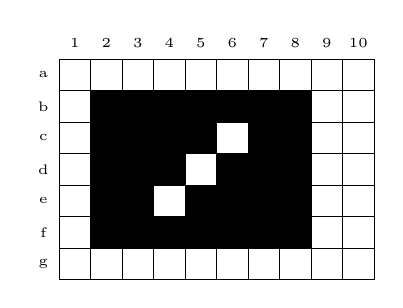
\begin{tikzpicture}[scale=0.4, every node/.style={inner sep=0.001}]
      \foreach \y [count=\n] in {
        {white,white,white,white,white,white,white,white,white,white},
        {white,black,black,black,black,black,black,black,white,white},
        {white,black,black,black,black,white,black,black,white,white},
        {white,black,black,black,white,black,black,black,white,white},
        {white,black,black,white,black,black,black,black,white,white},
        {white,black,black,black,black,black,black,black,white,white},
        {white,white,white,white,white,white,white,white,white,white},
      } {
        % Column labels & heatmap tiles
        \foreach \x [count=\m] in \y {
          \ifnum\n=1
            \node[minimum size=4mm] at (\m, 0) {\tiny \m};
          \fi
          \node[draw, fill=\x, minimum size=4mm] at (\m,-\n) {};
        }
      }

      % Row labels
      \foreach \a [count=\i] in {a,b,c,d,e,f,g} {
        \node[minimum size=4mm] at (0,-\i) {\tiny \a};
      }
    \end{tikzpicture}
    \caption{Black rectangle on the left side}\label{subfig:evtcams:evts_rel_motion:black_bf}
  \end{subfigure}
  \begin{subfigure}{0.475\linewidth}
    \centering
    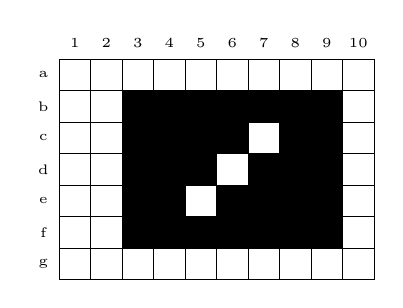
\begin{tikzpicture}[scale=0.4, every node/.style={inner sep=0.001}]
      \foreach \y [count=\n] in {
        {white,white,white,white,white,white,white,white,white,white},
        {white,white,black,black,black,black,black,black,black,white},
        {white,white,black,black,black,black,white,black,black,white},
        {white,white,black,black,black,white,black,black,black,white},
        {white,white,black,black,white,black,black,black,black,white},
        {white,white,black,black,black,black,black,black,black,white},
        {white,white,white,white,white,white,white,white,white,white},
      } {
        % Column labels & heatmap tiles
        \foreach \x [count=\m] in \y {
          \ifnum\n=1
            \node[minimum size=4mm] at (\m, 0) {\tiny \m};
          \fi
          \node[draw, fill=\x, minimum size=4mm] at (\m,-\n) {};
        }
      }

      % Row labels
      \foreach \a [count=\i] in {a,b,c,d,e,f,g} {
        \node[minimum size=4mm] at (0,-\i) {\tiny \a};
      }
    \end{tikzpicture}
    \caption{Black rectangle on the right side}\label{subfig:evtcams:evts_rel_motion:black_af}
  \end{subfigure}\\
  \vspace{3mm}
  \begin{subfigure}{0.475\linewidth}
    \centering
    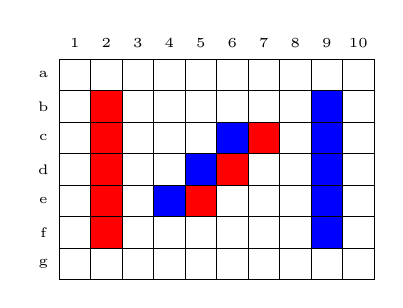
\begin{tikzpicture}[scale=0.4, every node/.style={inner sep=0.001}]
      \foreach \y [count=\n] in {
        {white,white,white,white,white,white,white,white,white,white},
        {white,  red,white,white,white,white,white,white, blue,white},
        {white,  red,white,white,white, blue,  red,white, blue,white},
        {white,  red,white,white, blue,  red,white,white, blue,white},
        {white,  red,white, blue,  red,white,white,white, blue,white},
        {white,  red,white,white,white,white,white,white, blue,white},
        {white,white,white,white,white,white,white,white,white,white},
      } {
        % Column labels & heatmap tiles
        \foreach \x [count=\m] in \y {
          \ifnum\n=1
            \node[minimum size=4mm] at (\m, 0) {\tiny \m};
          \fi
          \node[draw, fill=\x, minimum size=4mm] at (\m,-\n) {};
        }
      }

      % Row labels
      \foreach \a [count=\i] in {a,b,c,d,e,f,g} {
        \node[minimum size=4mm] at (0,-\i) {\tiny \a};
      }
    \end{tikzpicture}
    \caption{Events from (\subref{subfig:evtcams:evts_rel_motion:black_bf}) to (\subref{subfig:evtcams:evts_rel_motion:black_af})}\label{subfig:evtcams:evts_rel_motion:black_bf_to_af}
  \end{subfigure}
  \begin{subfigure}{0.475\linewidth}
    \centering
    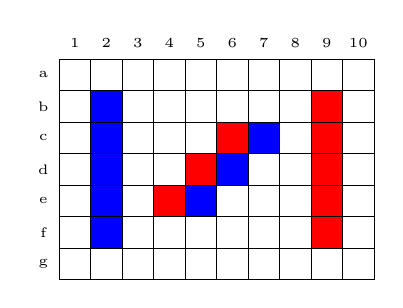
\begin{tikzpicture}[scale=0.4, every node/.style={inner sep=0.001}]
      \foreach \y [count=\n] in {
        {white,white,white,white,white,white,white,white,white,white},
        {white, blue,white,white,white,white,white,white,  red,white},
        {white, blue,white,white,white,  red, blue,white,  red,white},
        {white, blue,white,white,  red, blue,white,white,  red,white},
        {white, blue,white,  red, blue,white,white,white,  red,white},
        {white, blue,white,white,white,white,white,white,  red,white},
        {white,white,white,white,white,white,white,white,white,white},
      } {
        % Column labels & heatmap tiles
        \foreach \x [count=\m] in \y {
          \ifnum\n=1
            \node[minimum size=4mm] at (\m, 0) {\tiny \m};
          \fi
          \node[draw, fill=\x, minimum size=4mm] at (\m,-\n) {};
        }
      }

      % Row labels
      \foreach \a [count=\i] in {a,b,c,d,e,f,g} {
        \node[minimum size=4mm] at (0,-\i) {\tiny \a};
      }
    \end{tikzpicture}
    \caption{Events from (\subref{subfig:evtcams:evts_rel_motion:black_af}) to (\subref{subfig:evtcams:evts_rel_motion:black_bf})}\label{subfig:evtcams:evts_rel_motion:black_af_to_bf}
  \end{subfigure}\\
  \vspace{3mm}
  \begin{subfigure}{0.475\linewidth}
    \centering
    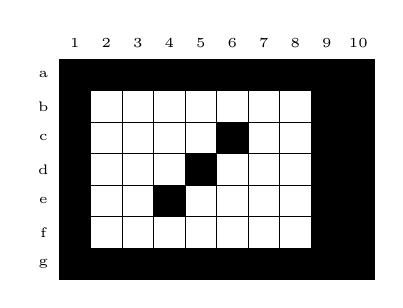
\begin{tikzpicture}[scale=0.4, every node/.style={inner sep=0.001}]
      \foreach \y [count=\n] in {
        {black,black,black,black,black,black,black,black,black,black},
        {black,white,white,white,white,white,white,white,black,black},
        {black,white,white,white,white,black,white,white,black,black},
        {black,white,white,white,black,white,white,white,black,black},
        {black,white,white,black,white,white,white,white,black,black},
        {black,white,white,white,white,white,white,white,black,black},
        {black,black,black,black,black,black,black,black,black,black},
      } {
        % Column labels & heatmap tiles
        \foreach \x [count=\m] in \y {
          \ifnum\n=1
            \node[minimum size=4mm] at (\m, 0) {\tiny \m};
          \fi
          \node[draw, fill=\x, minimum size=4mm] at (\m,-\n) {};
        }
      }

      % Row labels
      \foreach \a [count=\i] in {a,b,c,d,e,f,g} {
        \node[minimum size=4mm] at (0,-\i) {\tiny \a};
      }
    \end{tikzpicture}
    \caption{White rectangle on the left side}\label{subfig:evtcams:evts_rel_motion:white_bf}
  \end{subfigure}
  \begin{subfigure}{0.475\linewidth}
    \centering
    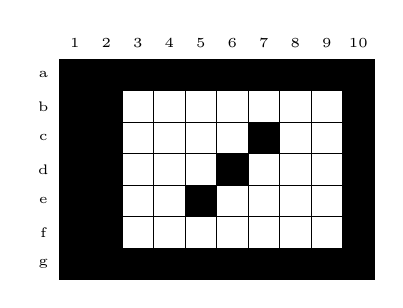
\begin{tikzpicture}[scale=0.4, every node/.style={inner sep=0.001}]
      \foreach \y [count=\n] in {
        {black,black,black,black,black,black,black,black,black,black},
        {black,black,white,white,white,white,white,white,white,black},
        {black,black,white,white,white,white,black,white,white,black},
        {black,black,white,white,white,black,white,white,white,black},
        {black,black,white,white,black,white,white,white,white,black},
        {black,black,white,white,white,white,white,white,white,black},
        {black,black,black,black,black,black,black,black,black,black},
      } {
        % Column labels & heatmap tiles
        \foreach \x [count=\m] in \y {
          \ifnum\n=1
            \node[minimum size=4mm] at (\m, 0) {\tiny \m};
          \fi
          \node[draw, fill=\x, minimum size=4mm] at (\m,-\n) {};
        }
      }

      % Row labels
      \foreach \a [count=\i] in {a,b,c,d,e,f,g} {
        \node[minimum size=4mm] at (0,-\i) {\tiny \a};
      }
    \end{tikzpicture}
    \caption{White rectangle on the right side}\label{subfig:evtcams:evts_rel_motion:white_af}
  \end{subfigure}\\
  \vspace{3mm}
  \begin{subfigure}{0.475\linewidth}
    \centering
    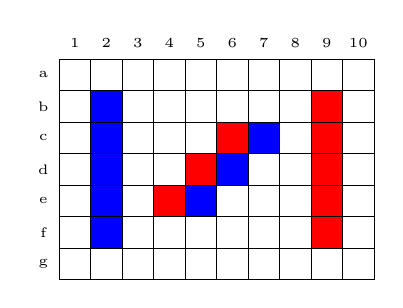
\begin{tikzpicture}[scale=0.4, every node/.style={inner sep=0.001}]
      \foreach \y [count=\n] in {
        {white,white,white,white,white,white,white,white,white,white},
        {white, blue,white,white,white,white,white,white,  red,white},
        {white, blue,white,white,white,  red, blue,white,  red,white},
        {white, blue,white,white,  red, blue,white,white,  red,white},
        {white, blue,white,  red, blue,white,white,white,  red,white},
        {white, blue,white,white,white,white,white,white,  red,white},
        {white,white,white,white,white,white,white,white,white,white},
      } {
        % Column labels & heatmap tiles
        \foreach \x [count=\m] in \y {
          \ifnum\n=1
            \node[minimum size=4mm] at (\m, 0) {\tiny \m};
          \fi
          \node[draw, fill=\x, minimum size=4mm] at (\m,-\n) {};
        }
      }

      % Row labels
      \foreach \a [count=\i] in {a,b,c,d,e,f,g} {
        \node[minimum size=4mm] at (0,-\i) {\tiny \a};
      }
    \end{tikzpicture}
    \caption{Events from (\subref{subfig:evtcams:evts_rel_motion:white_bf}) to (\subref{subfig:evtcams:evts_rel_motion:white_af})}\label{subfig:evtcams:evts_rel_motion:white_bf_to_af}
  \end{subfigure}
  \begin{subfigure}{0.475\linewidth}
    \centering
    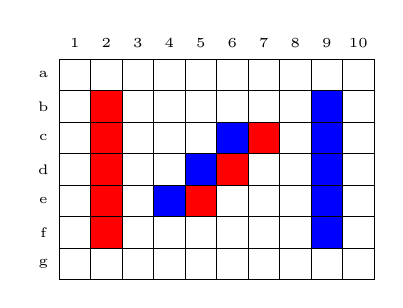
\begin{tikzpicture}[scale=0.4, every node/.style={inner sep=0.001}]
      \foreach \y [count=\n] in {
        {white,white,white,white,white,white,white,white,white,white},
        {white, red,white,white,white,white,white,white,  blue,white},
        {white, red,white,white,white,  blue, red,white,  blue,white},
        {white, red,white,white,  blue, red,white,white,  blue,white},
        {white, red,white,  blue, red,white,white,white,  blue,white},
        {white, red,white,white,white,white,white,white,  blue,white},
        {white,white,white,white,white,white,white,white,white,white},
      } {
        % Column labels & heatmap tiles
        \foreach \x [count=\m] in \y {
          \ifnum\n=1
            \node[minimum size=4mm] at (\m, 0) {\tiny \m};
          \fi
          \node[draw, fill=\x, minimum size=4mm] at (\m,-\n) {};
        }
      }

      % Row labels
      \foreach \a [count=\i] in {a,b,c,d,e,f,g} {
        \node[minimum size=4mm] at (0,-\i) {\tiny \a};
      }
    \end{tikzpicture}
    \caption{Events from (\subref{subfig:evtcams:evts_rel_motion:white_af}) to (\subref{subfig:evtcams:evts_rel_motion:white_bf})}\label{subfig:evtcams:evts_rel_motion:white_af_to_bf}
  \end{subfigure}
  \caption{Simple ``moving rectangle'' example. Each cell in the four grids represents a pixel. (\subref{subfig:evtcams:evts_rel_motion:black_bf})~A simple black rectangle on a white background, with an oblique line in its center. (\subref{subfig:evtcams:evts_rel_motion:black_af})~The same rectangle, one pixel to the right. (\subref{subfig:evtcams:evts_rel_motion:black_bf_to_af})~The events generated due to internal motion and/or camera motion, from the (\subref{subfig:evtcams:evts_rel_motion:black_bf}) to the (\subref{subfig:evtcams:evts_rel_motion:black_af}) situation ({\color{red}positive} events are in {\color{red}red}, {\color{blue}negative} ones in {\color{blue}blue}); notice how only the central oblique line and the left and right edges trigger events, as they are the only places where brightness values changed. (\subref{subfig:evtcams:evts_rel_motion:black_af_to_bf})~Like (\subref{subfig:evtcams:evts_rel_motion:black_bf_to_af}), but for the inverse motion; notice how the polarities have been inverted. (\subref{subfig:evtcams:evts_rel_motion:white_bf}) to (\subref{subfig:evtcams:evts_rel_motion:white_af_to_bf}): like (\subref{subfig:evtcams:evts_rel_motion:black_bf}) to (\subref{subfig:evtcams:evts_rel_motion:black_af_to_bf}), but for the inverse colors; notice how the the polarities have been inverted once again.}\label{fig:evtcams:evts_rel_motion}
\end{figure}

Furthermore, the output rate of a pixel (and therefore, of the whole event camera) is highly variable. In case of no or very few changes in the scene, the brightness values will remain almost constant, and thus little to no events will be fired. On the contrary, under highly varying light conditions or for highly dynamic scenes, the brightness values will vary greatly, leading to many events being fired.

A comparison between frames and events for a same scene is given in \cref{fig:evtcams:fan_rgb_vs_evts}, demonstrating all these principles for a practical example.

\begin{figure}
  \centering
  \begin{subfigure}{0.475\linewidth}
    \centering
    \includegraphics[width=\linewidth]{mainmatter/figures/2_event_cameras/fan_rgb_vs_evts/fan_rgb/plotted_frames.pdf}
    \caption{}\label{subfig:evtcams:fan_rgb_vs_evts:rgb}
  \end{subfigure}
  \begin{subfigure}{0.475\linewidth}
    \centering
    \includegraphics[width=\linewidth]{mainmatter/figures/2_event_cameras/fan_rgb_vs_evts/fan_evts/plotted_events.pdf}
    \caption{}\label{subfig:evtcams:fan_rgb_vs_evts:evts}
  \end{subfigure}\\
  \vspace{3mm}
  \begin{subfigure}{0.475\linewidth}
    \centering
    \includegraphics[width=\linewidth]{mainmatter/figures/2_event_cameras/fan_rgb_vs_evts/fan_evts/plotted_events_front.pdf}
    \caption{}\label{subfig:evtcams:fan_rgb_vs_evts:evts_front}
  \end{subfigure}
  \caption{Comparison between frames and events for a simple ``Rotating fan'' sequence. (\subref{subfig:evtcams:fan_rgb_vs_evts:rgb})~Even with a 300\acrshort{fps} camera, only four frames are captured over the course of 10ms, all showcasing motion blur and motion discontinuity for the blades, as well as redundant background information. (\subref{subfig:evtcams:fan_rgb_vs_evts:evts})~In comparison, with an event camera, the full motion of the blades can be acquired: each dot is an event, color-coded according to its timestamp for a better visualization. (\subref{subfig:evtcams:fan_rgb_vs_evts:evts_front})~A front view of (\subref{subfig:evtcams:fan_rgb_vs_evts:evts}) is given to better showcase the motion continuity property of the event camera in a frame-like visualization.}\label{fig:evtcams:fan_rgb_vs_evts}
\end{figure}

\section{Advantages and Challenges}
Due to their unique working principle, event cameras have many advantages when compared to more traditional sensors, but they also come with some notable drawbacks.

\subsection{Advantages}

\paragraph{Asynchrony}
The main advantage of event cameras compared to their frame-based counterpart is that they do not rely on a synchronous sampling of the scene. Instead, brightness changes are detected and transmitted as soon as they happen. This way, the information of what is happening in the scene can be known with a very low latency. In addition, the problems of motion blur and of under-/over-exposure are eliminated, since they are both consequences of the light accumulation process in frame-based cameras.

\paragraph{\acrfull{hdr}}
Whereas most frame-based cameras are restricted to a dynamic range of 40 to 60dB, event cameras can reach a dynamic range of more than 120dB~\cite{Finateu2020510A1}. This is due to the two intrinsic properties of the event camera: working in the logarithmic framework, and not being limited by exposure issues since they do not rely on an accumulation process. This high dynamic range makes them able to see under very dark or very bright conditions, e.g., during nighttime or in broad daylight.

\paragraph{Low Energy Consumption}
As they only capture and transmit brightness changes, i.e., non-redundant information, most event cameras have a power consumption of under 100mW (20 times less than comparable frame-based cameras), making them particularly suited for low-power embedded systems.

\subsection{Challenges}

\paragraph{Change of Paradigm}\label{sec:evtcams:adv_chall:chall:paradigm}
The main challenge with event cameras is that they propose a completely novel paradigm. As such, most of the frame-based literature and algorithms proposed over the past decades have to be entirely revamped. In addition, computers and \acrshortpl{gpu} are better suited to process synchronous dense matrix-based data like frames, rather than sparse and asynchronous event-based data.

\paragraph{Noise}
Since event cameras do not rely on a temporal accumulation process, they are much more sensitive to noise than frame-based cameras. This will result in events being triggered without a corresponding brightness change, or on the contrary, events being missed. This noise comes from different sources: \gls{shot_noise}, internal circuits noise, \glspl{hot_pixel}, etc.

\paragraph{Output Rates}
As noted earlier, the output rate of an event camera is highly variable. While the output rate of a frame-based camera is predetermined (up to 300\acrshort{fps} for high-speed cameras), event cameras can reach output rates of up to millions of events per sec for \acrshort{hd} sensors. Designing methods able to handle such rates in real-time is one of the most critical issues with event cameras.

\paragraph{Lack of Absolute Brightness Values}
As shown in \cref{eq:evtcams:delta_l,eq:evtcams:delta_l_thr}, events only provide information about relative brightness changes. No reference absolute brightness value is available, meaning that some problems like frame reconstruction from events alone are particularly difficult. To circumvent this issue, some camera models offer both the frame and event modalities in a single sensor~\cite{Brandli2014A2,Posch2011AQ1}. However, adding this frame modality is currently limited to low- or mid-resolution cameras, and it results in a more noisy event stream due to electrical interferences between both circuits.

\section{Application to Intelligent Robotics}
As noted in the introduction to this thesis (\cref{sec:intro:context}), intelligent robotic systems operating in open environments are in a critical need of novel sensors and methods able to work even in the most complex conditions. Intelligent vehicles are particularly concerned, as for instance they should be able to quickly detect a pedestrian at night even on non-illuminated roads. As such, event cameras may represent a sensor of choice, as they provide answers to the most predominant issues encountered with frame-based cameras.

\paragraph{Independence to Lighting Conditions}
The high dynamic range of the event cameras allows them to observe scenes even with low or with very high illumination. In the case of intelligent vehicles, these conditions are typically met when driving during night, or when the sun is facing the windshield at dawn and dusk. A mixture of both low and high illumination can also be encountered, for instance at the exit of a tunnel, and frame-based cameras are notorious for producing bad results under these conditions.

\paragraph{Low Reaction Times}
Their asynchronous response to brightness changes and their low latency allows for the design of novel methods with very low reaction times. Such reaction times are particularly critical when operating in open environments, as external vulnerable users may always appear unexpectedly, requiring quick evasive maneuvering.

\paragraph{Absence of Motion Blur}
The lack of any motion blur is also critical, as the ego-motion of the robot or the motion of the objects in the scene does not introduce additional noise, and therefore makes their detection and identification easier.

\section{Review of the State of the Art}
We give in this section a quick review of the current state of the art. The objective is not to be exhaustive, but rather to give the reader an overview of the work achieved so far using event cameras. More detailed reviews of the state of the art will be given in each of the following chapters of this thesis for the corresponding issues. Yet, if the reader is interested, a complete review of the domain published in 2020 is available in~\cite{Gallego2020EventbasedVA}, and a more recent deep-learning-centered survey on event-based vision is available in~\cite{Zheng2023DeepLF}.

\subsection{Representations}
One of the main questions in the literature is about how to represent events to treat them efficiently. We list here some of the most common representations.

\paragraph{Raw Stream}
Some authors (for instance, \cite{Weikersdorfer2012EventbasedPF,Gallego2016EventBased6C,Gruel2022NeuromorphicES}) use directly the raw stream of events, and treat each of them individually, allowing for a fully event-based processing philosophy. This approach is the most conservative, as no information is lost by converting to another representation. However, it is also highly inefficient, due to the sparsity of the event data.

\paragraph{Time Surface}
The Time Surface~\cite{Delbrck2008FramefreeDD,Lagorce2017HOTSAH} is a simple representation of events as a 2D image. Constructed over a short temporal window of events, each pixel of the Time Surface is given the timestamp of the most recent event. This formulation allows for a simple conversion of event-based problems into a frame-based equivalent. However, the Time Surface is a lossy representation, as only the most recent event for each pixel is kept.

\paragraph{Event Volume}
The Event Volume~\cite{Zhu2019UnsupervisedEL,Perot2020LearningTD} keeps both the spatial and temporal information of events by storing them as a 3D tensor, especially adapted for learning-based approaches. While the full spatial resolution of the events is kept, timestamps are interpolated to place them in the adequate channels of the tensor, at the expense of some precision loss. In the original version of Zhu \textit{et al.}~\cite{Zhu2019UnsupervisedEL}, events of negative and positive polarities are added together, leading to some additional information loss. The formulation of Perot \textit{et al.}~\cite{Perot2020LearningTD} splits them in separate channels to avoid this issue, but results in a heavier representation.

\paragraph{Learned Representation}
More recently, some authors~\cite{Gehrig2019EndtoEndLO,Zubic2023FromCC} have started advocating for the learning of the event-based representation itself. The intrinsic idea is that, even though the Time Surface or the Event Volume are easily understandable by humans, they might not be the most adapted for neural networks. Optimizing automatically the event-based formulation allows for task-specific representations to appear, which only keep the required data. While these representations are harder to interpret, they have been proven to improve state-of-the-art performance in several tasks.

\paragraph{Reconstructed Images}
Finally, some authors~\cite{Scheerlinck2018ContinuoustimeIE,Rebecq2021HighSA,Dauner2023FromCC} reconstruct full images from the event stream. While this process is highly inefficient, it allows for the reuse of proven methods from the frame-based state of the art, yielding accurate results in numerous tasks.


\subsection{Processing Strategies}
Three main strategies are used across the literature to process events: filter-based, geometry-based, and learning-based methods.

\paragraph{Filter-Based Methods}
In the spirit of keeping a fully event-based processing methodology, some authors use individual events to update a central state using a filter-based approach. This strategy allows for a fully asynchronous processing of the event stream, and is particularly well-suited to the low amount of information each event can bring. In the case of~\cite{Scheerlinck2018ContinuoustimeIE}, a filter-based approach is used for reconstructing images at a high rate: images from a DAVIS~\cite{Brandli2014A2} camera are used as an optional state initialization, and events from the same camera are used to update this state to recreate subsequent images.

\paragraph{Model-Based Methods}
Model-based approaches aim at finding an optimal solution to a theoretical model of the considered problem which could be explained by the input data. In the case of event data, model-based methods are often applied on 2D images of events, using classical image processing algorithms, or directly on spatio-temporal 3D point clouds of events, using 3D-geometry-based or graph-based algorithms. For instance, Benosman \textit{et al.}~\cite{Benosman2014EventBasedVF} used a 3D plane-fitting algorithm to estimate the motion of events with respect to time.

\paragraph{Learning-Based Methods}
As in numerous other domains, learning-based methods have revolutionized event-based computer vision. Their natural capacity of learning from data directly allows them to provide accurate results even for the most complex tasks, and allows them to circumvent limitations with more traditional model-based methods (noise, missing or ambiguous data, \dots). Network architectures originally developed for frame-based computing have been proven to be also efficient for event-based tasks~\cite{Zhu2018EVFlowNetSO,Gehrig2021CombiningEA}, at the expense of requiring event data to be accumulated in a frame- or tensor-like representation. \Acrfullpl{snn} are an alternative approach~\cite{ParedesValls2021SelfSupervisedLO,Ranon2021StereoSpikeDL}, which allow for a sparse processing of the event data, but which require specific hardware to be trained efficiently. More recently, \acrfullpl{gnn} have started to be used with events~\cite{Alkendi2021NeuromorphicCD,Schaefer2022AEGNNAE}, as they represent explicitly relations between events while keeping their sparsity, and as they can be trained on standard \acrshortpl{gpu}.


\subsection{Applications}
More than 30 years after their inception~\cite{Mahowald1991TheSR,Mahowald1992VLSIAO}, event cameras have been applied to virtually every domain in computer vision. We list here some of their most popular applications.

\paragraph{Optical Flow}
Information encoded by an event camera is intrinsically linked to motion, as only the parts of the scenes which change along time due to motion of objects in the scene or of the camera itself create events. Therefore, optical flow constitutes one of the most explored issues in the event-based literature. While initial works were focused on sparse, per-event optical flow on limited motions~\cite{Benosman2014EventBasedVF,Stoffregen2017SimultaneousOF}, most recent works are able to compute dense optical flow maps in all types of scenes~\cite{Gehrig2021DenseOF,Liu2023TMATM}.

\paragraph{Disparity / Depth Estimation}
As with frame-based cameras, disparity / depth estimation is a very popular topic with event cameras. While many works use a stereo pair of event cameras~\cite{Schraml2010DynamicSV,Schraml2016AnES,Nam2022StereoDF}, other works have tried to estimate depth from the fusion of events with a different secondary modality (RGB~\cite{Gehrig2021CombiningEA}, RGB-D~\cite{Weikersdorfer2014Eventbased3S}, LiDAR~\cite{Li2021Enhancing3L,Cui2022DenseDE}), or from a single monocular event camera~\cite{Zhu2019UnsupervisedEL,Kim2016RealTime3R,HidalgoCarrio2020LearningMD}.

\paragraph{High Framerate \acrshort{hdr} Video}
Since event cameras are able to provide relative brightness change information at a very rate and with a high dynamic range, it is technically possible to ``revert'' the event generation process to recreate images at a very high framerate and in \acrshort{hdr}. While early methods~\cite{Scheerlinck2018ContinuoustimeIE} still required images as initial absolute brightness references, more recent methods~\cite{ParedesValls2021BackTE,Yu2022LearningTS,Ercan2023HyperE2VIDIE} have been able to circumvent this requirement by using learning-based approaches.

\paragraph{Object Detection and Tracking}
Thanks to their high frequency and low latency, event cameras are a sensor of choice for detecting and tracking objects in dynamic scenes. While initial works were focused on the recognition of simple shapes~\cite{SerranoGotarredona2009CAVIARA4,Wiesmann2012EventdrivenES}, more recent works are able to harness the power of learning-based methods to detect complex objects like vehicles or pedestrians~\cite{Perot2020LearningTD,Sironi2018HATSHO,Gehrig2022RecurrentVT}.


\subsection{State-of-the-Art Datasets}\label{sec:evtcams:sota:datasets}
Datasets are an important requirement, both for popularizing the event camera and making recordings available to the greatest number, and for providing benchmarks for evaluating event-based methods. In this era of dominance of neural networks, large datasets are also a critical need for training these networks efficiently. We list here the three main categories of event-based datasets: real-life, simulated, and converted frame-based datasets.

\paragraph{Converted Frame-Based Datasets}
Early works~\cite{Orchard2015ConvertingSI,Tan2015BenchmarkingNV} with event cameras tried to exploit the large amount of frame-based datasets available in the literature. To do so, an event camera was placed in front of a screen, where the videos or images from these datasets were displayed. In case of static images, the event camera was manually shaken to still display events. More recent works~\cite{Gehrig2019VideoTE,Hu2021v2eFV,Joubert2021EventCS} have tried to convert directly frame-based videos into their event-based equivalent, by extracting brightness changes along time. This method however requires a temporal upsampling of the video for more realistic timestamps, but results in the introduction of artifacts and errors compared to a real event camera.

\paragraph{Real-Life Datasets}
Following the wider availability of event cameras, numerous real-life datasets were recorded and published during the past decade. While early works were focused on simple and specific tasks (identification of playing cards~\cite{SerranoGotarredona2015PokerDVSAM}, recognition of gestures~\cite{Amir2017ALP}, \dots), more recent works have started to build long, complex, multitask datasets. Automotive datasets~\cite{Perot2020LearningTD,Zhu2018TheMS,Gehrig2021DSECAS,Chaney2023M3EDMM} are especially popular, as they can showcase highly varying environmental conditions (lighting, weather, traffic, \dots), and offer a wide range of problems to solve (sensor fusion, pose estimation, optical flow, object detection and recognition, semantic segmentation, \dots).

\paragraph{Simulated Datasets}
While real-life datasets are particularly useful, they often have limitations: partial and/or approximate ground truths, difficulties to synchronize and calibrate the sensors, lack of variety, few edge cases, etc. In comparison, fully simulated datasets can have a perfect ground truth, synchronization, and calibration, and can place the event camera in a wider range of situations. Several simulators~\cite{Mueggler2016TheED,Li2018InteriorNetMM,Rebecq2018ESIMAO} were proposed along the years, relying on the frame-to-event methods, but generating traditional frames at a high rate so that no temporal upsampling of the frame-based data is required. A model of the event camera was especially included in the automotive CARLA simulator~\cite{Dosovitskiy2017CARLAAO}, based on the work of Rebecq \textit{et al.}~\cite{Rebecq2018ESIMAO}.


\section{Popular Event Camera Models}
In this thesis, we will consider mainly three event camera models, which were used as part of the datasets of the thesis: the DAVIS346, Prophesee Gen3.1, and Prophesee Gen4 cameras.

\subsection{DAVIS346}
The DAVIS~\cite{Brandli2014A2} camera was initially released in 2014. Designed by iniVation\footnote{\url{https://inivation.com}}, this camera is one of the first event-based sensor prototype which was made available to the public (after the DVS128~\cite{Lichtsteiner2008A11} in 2008). In its DAVIS346 version, this sensor only has a resolution of \(346\text{px} \times 260\text{px}\), but is able of a high dynamic range of 120dB, a temporal resolution of 1\textmu{}s, a typical latency under 1ms, and it is able to produce at most 12\acrshort{meps}.

In addition to the event-based modality, the DAVIS346 camera also embarks a frame-based sensor, sharing the same pixels than the event-based sensor. Despite only being able to produce grayscale frames at the same low resolution of \(346\text{px} \times 260\text{px}\) and with only a maximum frame rate of 40\acrshort{fps}, this secondary modality was an achievement at the time. It allowed for the first comparisons of frame-based and event-based methods, for a better comprehension of the strengths and weaknesses of the event-based modality, and for the apparition of novel methods based on the fusion of frames and events.

\subsection{Prophesee Gen3.1}
The Prophesee Gen3.1 sensor was released in early 2020. Designed by Prophesee\footnote{\url{https://www.prophesee.ai}}, it has a resolution of \(640\text{px} \times 480\text{px}\) (VGA), a high dynamic range of above 120dB, a typical latency of 200\textmu{}s, and can output at most 50\acrshort{meps}.

While it does not embark a frame-based modality, the Prophesee Gen3.1 camera constituted an interesting upgrade in terms of resolution from the DAVIS cameras. As such, it was included in multiple datasets, like DSEC~\cite{Gehrig2021DSECAS} and EVIMO2~\cite{Burner2022EVIMO2AE}.

\subsection{Prophesee Gen4}
The Prophesee Gen4~\cite{Finateu2020510A1} camera was released in mid-2020. Also designed by Prophesee, this camera is one of the first high definition event sensor, with a resolution of \(1280\text{px} \times 720\text{px}\). Similarly to the DAVIS346 and Prophesee Gen3.1 cameras, the Prophesee Gen4 has a high dynamic range (above 124dB), a high bandwidth (up to 1066\acrshort{meps}), and a low latency (between 20 and 150\textmu{}s).

As will be shown in the following sections of this thesis, the availability of high definition event sensor was becoming a critical need. Events from low- and mid-resolution sensors lack detail, leading to low performances for applications which rely on precise object edges and/or textures (e.g., object recognition), but remain popular for low-power embedded systems (like the Prophesee GenX320 sensor~\cite{Prophesee2023IntroducingTW} for \acrshort{ar}/\acrshort{vr}). However, the higher level of details of high definition event cameras brings new issues, in particular a much higher event throughput which becomes harder to treat in real time.

\section{Datasets}\label{sec:evtcams:datasets}
As noted in \cref{sec:evtcams:sota:datasets}, datasets including the event-based modality have been an increasing need over the past decade. This need has been further reinforced with the arrival of learning-based methods, which require large amounts of data to be trained. In this section, we give a more detailed focus on three datasets of the state of the art, which were used throughout the thesis: the MVSEC~\cite{Zhu2018TheMS}, DSEC~\cite{Gehrig2021DSECAS}, and M3ED~\cite{Chaney2023M3EDMM} datasets. A summary of the content of these datasets is given in \cref{tab:evtcams:datasets}.

\begin{table}[ht]
  \centering
  \resizebox{\linewidth}{!}{
    \begin{tabular}{@{}lccc@{}}
      \toprule
      & MVSEC & DSEC & M3ED \\
      \midrule
      Year & 2018 & 2021 & 2023 \\
      \midrule
      \multirow{2}{*}{Event data} & 2\texttimes{} DAVIS346 & 2\texttimes{} Prophesee Gen3.1 & 2\texttimes{} Prophesee Gen4 \\
      & (346\texttimes{}260) & (640\texttimes{}480) & (1280\texttimes{}720) \\
      \midrule
      \multirow{4}{*}{Images} & 2\texttimes{} DAVIS346 \\
      & (346\texttimes{}260) & 2\texttimes{} FLIR Blackfly S & OVC 3b (3 cameras) \\
      \cmidrule(lr){2-2}
      & 2\texttimes{} VI-Sensor & (1440\texttimes{}1080, 20Hz) & (1280\texttimes{}800) \\
      & (752\texttimes{}480, 20Hz) \\
      \midrule
      \multirow{3}{*}{LiDAR data} & Velodyne VLP-16 & Velodyne VLP-16 & Ouster OS1-64U \\
      & (16 channels, 100m range, &  (16 channels, 100m range, & (64 channels, 120m range, \\
      & 20Hz, 30\textdegree{} vertical FOV) & 10Hz, 30\textdegree{} vertical FOV) & 10Hz, 45\textdegree{} vertical FOV) \\
      \midrule
      \multirow{2}{*}{Types of scene} & Drone, handheld, & \multirow{2}{*}{Car} & Drone, car, \\
      & car, motorcycle & & legged robot \\
      \midrule
      Day and night & Yes & Yes & Yes \\
      \midrule
      \multirow{2}{*}{Ground truth data} & Pose, semi-dense depth, & Pose, semi-dense disparity, semi-dense optical flow, & Pose, sparse depth, \\
      & semi-dense optical flow & dense semantic maps, 2D bounding boxes & dense semantic maps, 3D bounding boxes \\
      \midrule
      Total duration & 1 hour & 53 hours & 200 hours \\
      \midrule
      Train/val/test sets? & No & Yes & Yes \\
      \bottomrule
    \end{tabular}
  }
  \caption{Comparison of the state-of-the-art datasets used throughout the thesis.}\label{tab:evtcams:datasets}
\end{table}

\subsection{MVSEC}\label{sec:evtcams:datasets:mvsec}
The Multivehicle Stereo Event Camera (MVSEC) dataset~\cite{Zhu2018TheMS} was recorded in 2018. It contains data from multiple sensors: low-resolution (346\texttimes{}260) events and images from two DAVIS346 cameras, higher-resolution (752\texttimes{}480) images from two VI-Sensor cameras, IMU measurements from both the DAVIS346 and VI-sensor cameras, point clouds from a 16-channel Velodyne LiDAR, and GPS data from a UBlox receiver. In total, the MVSEC dataset is composed of four types of sequences, for more than 1 hour of data: 6 short flying sequences, 2 handheld sequences, 5 long outdoor driving sequences, and a single long motorcycle riding sequence.

This dataset was originally intended for depth and pose estimation, as its authors offer semi-dense ground truth depth maps and groud truth reference poses. Yet, following subsequent work~\cite{Zhu2018EVFlowNetSO}, they were also able to compute semi-dense ground truth optical flow maps, by using the depth maps and the poses.

However, as highlighted by its authors~\cite{Zhu2018TheMS}, this dataset suffers from multiple flaws: the data is loosely synchronized, the biases of the event cameras were not adjusted, the calibration is approximate, and moving objects in the scene create errors in the ground truth data. For this last point in particular, the authors of MVSEC accumulate consecutive point clouds to construct a dense view of the scene, which is then reprojected in 2D to construct the ground truth depth maps. However, if an element moves in the scene during the accumulation period, then it will appear ``blurry'' in the accumulated view, leading to errors in both the ground truth depth maps and optical flow maps. This issue is particularly critical, as the driving sequences contain many moving vehicles and pedestrians. Yet, MVSEC remains the most popular dataset for both depth estimation and optical flow, and as such constitutes an interesting benchmark for the thesis work.

\subsection{DSEC}
The Stereo Event Camera Dataset for Driving Scenarios (DSEC)~\cite{Gehrig2021DSECAS} was recorded in 2021. It contains data from mid-resolution (640\texttimes{}480) events from two Prophesee Gen3.1 cameras, high-definition (1440\texttimes{}1080) images from two FLIR Backfly S cameras, point clouds from a 16-channel Velodyne LiDAR, and GPS data from a UBlox receiver. In total, the DSEC dataset is composed of 53 sequences of day and night driving, for more than 53 hours of data.

This dataset was originally intended for disparity and depth estimation, as its authors offer semi-dense ground truth disparity maps. However, the DSEC dataset received several extensions, and now offers ground truth semi-dense optical flow maps~\cite{Gehrig2021DenseOF}, dense semantic segmentation maps~\cite{Sun2022ESSLE}, and 2D bounding boxes for pedestrians and vehicles~\cite{Gehrig2022PushingTL}.

\subsection{M3ED}
The Multi-Robot, Multi-Sensor, Multi-Environment Event Dataset (M3ED)~\cite{Chaney2023M3EDMM} was recorded in 2023, and acts as an informal successor to the MVSEC dataset. It contains data from high-definition (1280\texttimes{}720) events from two Prophesee Gen4 cameras, high-definition (1280\texttimes{}800) images from three cameras mounted on an OVC 3b platform, point clouds from a 64-channel Ouster LiDAR, and GPS data from a UBlox receiver. In total, the M3ED dataset is composed of three types of sequences, for more than 200 hours of data: 40 indoor and outdoor sequences filmed with an \acrshort{uav} and with a legged robot, and 17 outdoor driving sequences.

Like the MVSEC dataset, M3ED is mainly intended for depth and pose estimation, as its authors offer sparse ground truth depth maps and ground truth reference poses. However, following the extensions of the DSEC dataset, they also offer dense 2D semantic maps, as well as 3D bounding boxes for pedestrians, buildings, cars, and trees.

One of the key elements of the M3ED dataset is that its authors have fixed the issue of the incorrect depths for the moving objects of the MVSEC dataset, by identifying them and discarding erroneous values automatically. Yet, their conservative approach also tends to discard correct data, resulting in very sparse ground truth depth maps.
